% =============================================================
%  SECTION: Module 3 — The Velocity Verlet Integrator
%  ASSIGNED TO: [Person Name]
%
%  GUIDING QUESTIONS TO ANSWER:
%   WHAT  — What is numerical integration? What does Velocity Verlet do?
%   WHY   — Why can't we solve the equations of motion analytically?
%           Why Velocity Verlet over, say, simple Euler integration?
%   HOW   — Walk through the 4-step VV algorithm.
%           How is energy conservation used as a reliability check?
%  EXTRAS — What is a "good" time step? The 1-in-10^4 fluctuation rule.
%           What does energy drift look like when dt is too large?
%           What is the reduced time unit t* and how is dt chosen?
% =============================================================

\newpage
\section{Module 3: The Velocity Verlet Integrator}

\subsection{What Are We Doing?}
% We need to evolve atomic positions and velocities forward in time.
% Since forces change constantly, there's no closed-form solution → finite differences.
% [WRITE HERE]

\subsection{Why Are We Doing It?}

\subsubsection{Why Can't We Solve This Analytically?}
% N coupled, nonlinear ODEs. Positions affect forces, forces affect positions.
% No analytical solution for N > 2. Must discretise time.
% [WRITE HERE]

\subsubsection{Why Velocity Verlet?}
% Compare to simple Euler: VV is time-reversible, symplectic (conserves phase volume),
% and synchronises positions and velocities at the same time step.
% Euler accumulates error; VV oscillates around the true energy without drift.
% [WRITE HERE — intuition is key here]

\subsection{How Is It Implemented?}

\subsubsection{The Algorithm}

The Velocity Verlet update proceeds in four steps per timestep $\delta t^*$:

\begin{enumerate}
    \item \textbf{Update positions:}
    \begin{equation}
        \mathbf{r}_i(t+\delta t) = \mathbf{r}_i(t) + \mathbf{v}_i(t)\,\delta t + \tfrac{1}{2}\mathbf{a}_i(t)\,\delta t^2
        \label{eq:vv_pos}
    \end{equation}

    \item \textbf{Half-step velocity:}
    \begin{equation}
        \mathbf{v}_i\!\left(t + \tfrac{1}{2}\delta t\right) = \mathbf{v}_i(t) + \tfrac{1}{2}\mathbf{a}_i(t)\,\delta t
        \label{eq:vv_vhalf}
    \end{equation}

    \item \textbf{Recalculate forces} from new positions (Module 1 + 2 logic).

    \item \textbf{Complete velocity update:}
    \begin{equation}
        \mathbf{v}_i(t + \delta t) = \mathbf{v}_i\!\left(t + \tfrac{1}{2}\delta t\right) + \tfrac{1}{2}\mathbf{a}_i(t+\delta t)\,\delta t
        \label{eq:vv_vfull}
    \end{equation}
\end{enumerate}

In reduced units, $m^* = 1$, so $\mathbf{a}_i^* = \mathbf{F}_i^*$.

\subsubsection{Choosing the Time Step}

The reduced time unit is $t^* = t/t_0$ where $t_0 = \sigma\sqrt{m/\eps}$. A good rule of thumb is to have $\sim50$ timesteps per vibrational period. For the LJ system we use $\delta t^* = 0.005$. The stability criterion is:
\begin{equation}
    \frac{\Delta E^*}{\langle E^* \rangle} \lesssim 10^{-4}
\end{equation}
where $\Delta E^*$ is the fluctuation in total energy during the production run.

\subsubsection{Kinetic and Potential Energy}

In reduced units ($m^* = 1$):
\begin{align}
    K^* &= \frac{1}{2}\sum_{i=1}^{N} |\mathbf{v}_i^*|^2 \label{eq:ke}\\
    E^* &= K^* + U^* \label{eq:etot}
\end{align}

\subsection{Test Results}

% Run a short simulation (e.g. 200 steps) of a 2-atom or 32-atom system.
% Plot E*, K*, U* vs time step.
% Confirm total energy is flat (no drift), KE and PE oscillate but compensate.

\begin{figure}[H]
    \centering
    % 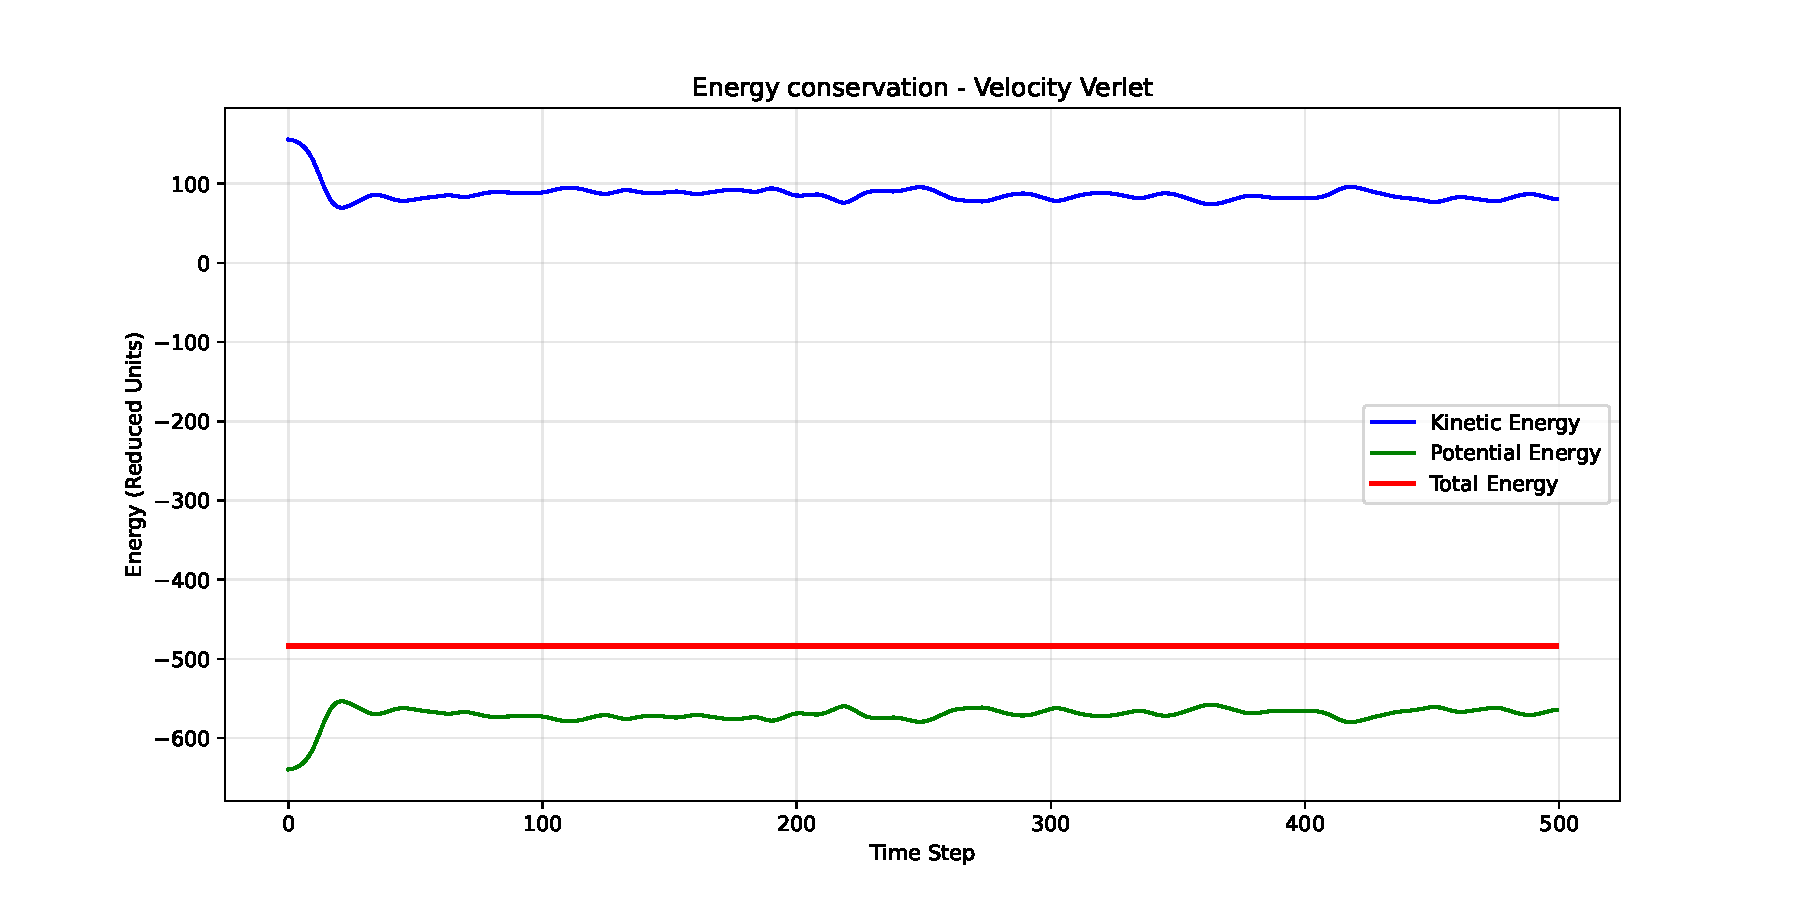
\includegraphics[width=\linewidth]{figures/m3_energy_conservation.pdf}
    \caption{Total energy $E^*$, kinetic energy $K^*$, and potential energy $U^*$ over time for a test run using the Velocity Verlet integrator with $\delta t^* = 0.005$. The total energy shows no systematic drift, confirming the integrator is working correctly.}
    \label{fig:m3_energy}
\end{figure}

% Report: mean E*, standard deviation of E*, ratio std/mean (should be ~1e-4 or better).
% [WRITE QUANTITATIVE RESULTS HERE]
